\section*{Branching Ratio}

The first step to evaluate the branching ratio between o-Ps and p-Ps consisted in the selection of the correct decay channel by mean of detectors geometry and signals coincidence.
As above mentioned p-Ps decays with the emission of two collinear photons with the same energy, due to the fact that positronium annihilation occurs essentially at rest, while o-Ps, for the same reason, decays with the emission of three coplanar photons, with an emission angle between them dependent on their energy.

In order to select the p-Ps decay channel, an angle of 180$^\circ$ was imposed between two of the three detectors on the goniometer~(see Fig~\ref{Fig:PsGeometry}-\emph{a}), and their coincidence was used as trigger signal for the digitizer. 

The o-Ps decay channel was selected, instead, placing the three detectors at 120$^\circ$ between them~(see Fig~\ref{Fig:PsGeometry}-\emph{b}) and using the triple coincidence as trigger signal for the digitizer. A longer acquisition time with respect to the first configuration was necessary due to the lower counter rate.

 
\begin{figure}[h!]
	\centering
	\subfloat[][\emph{p-Ps geometry}.]
	{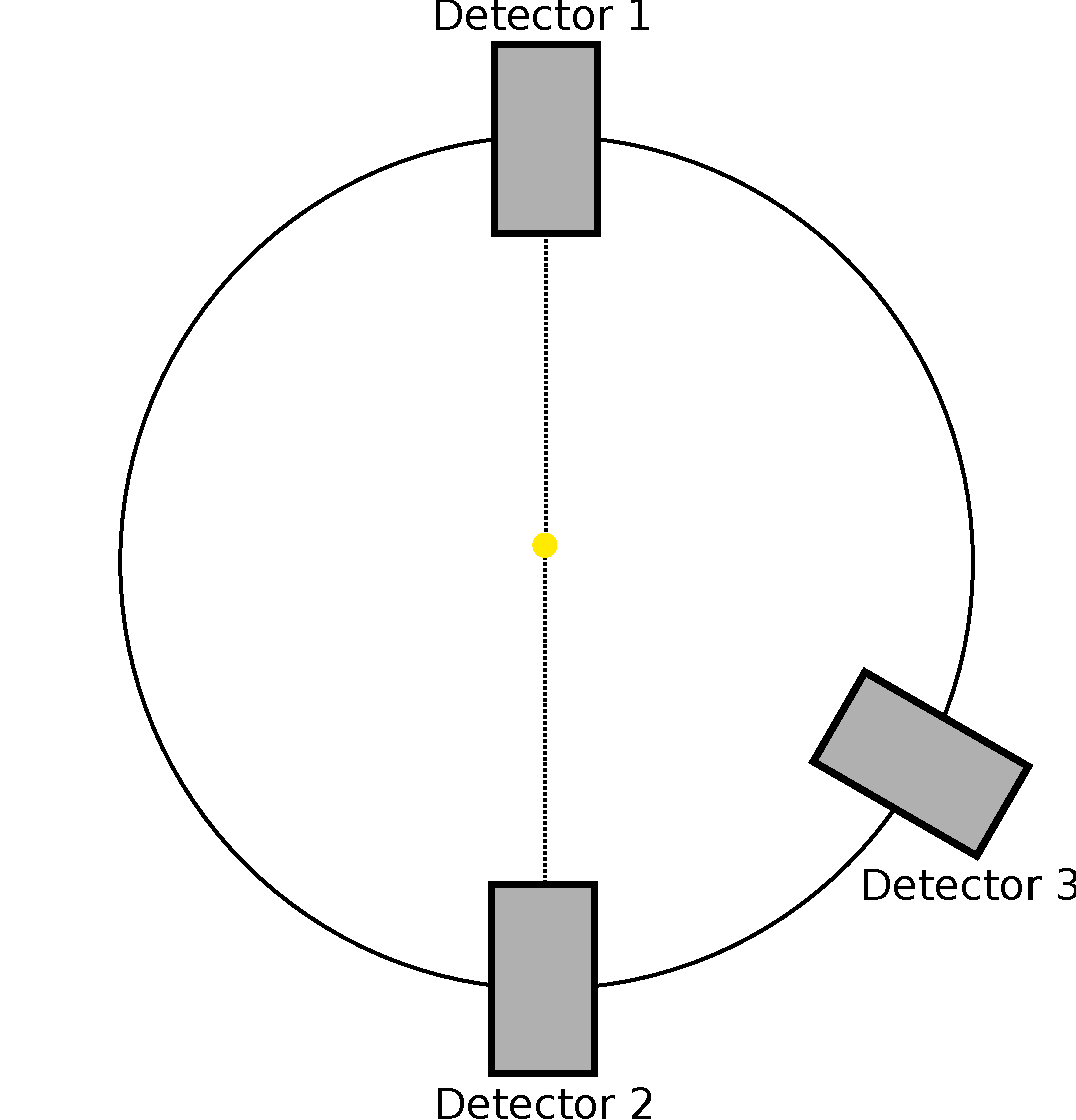
\includegraphics[width=.45\textwidth]{pPsGeometry}} \quad
		\subfloat[][\emph{o-Ps geometry}.]
	{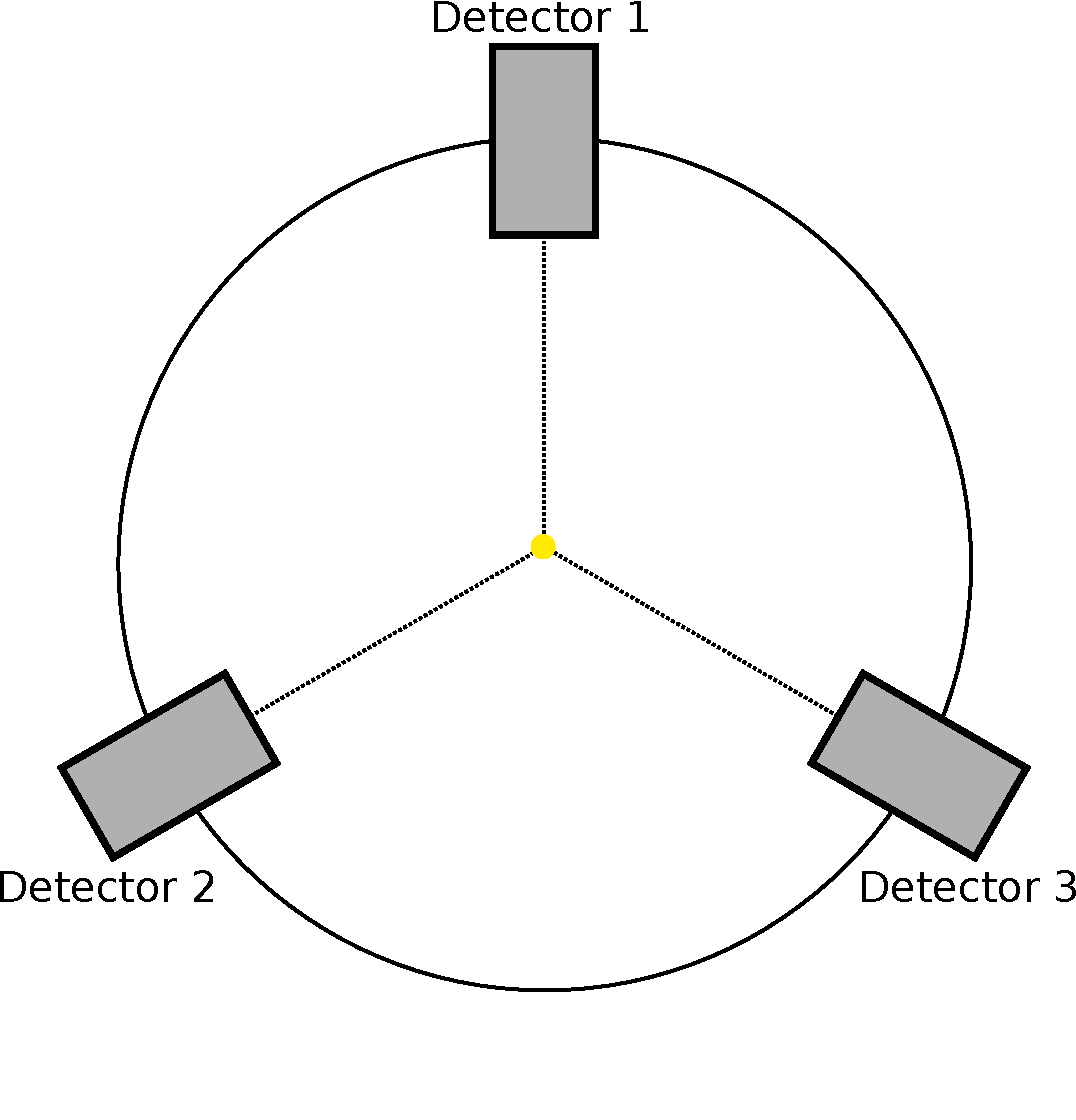
\includegraphics[width=.45\textwidth]{oPsGeometry}} \\
	\caption{Geometry of the experimental setup chosen for the p-Ps~(\emph{a}) and o-Ps~(\emph{b}) decay channel selection.}
	\label{Fig:PsGeometry}
\end{figure}

The spectra recorded by the two detectors for the p-Ps configuration are presented in Fig. \ref{Fig:1_2_spectra}.

\begin{figure}[H]
	\centering
	\subfloat[][\emph{Detector 1}.]
	{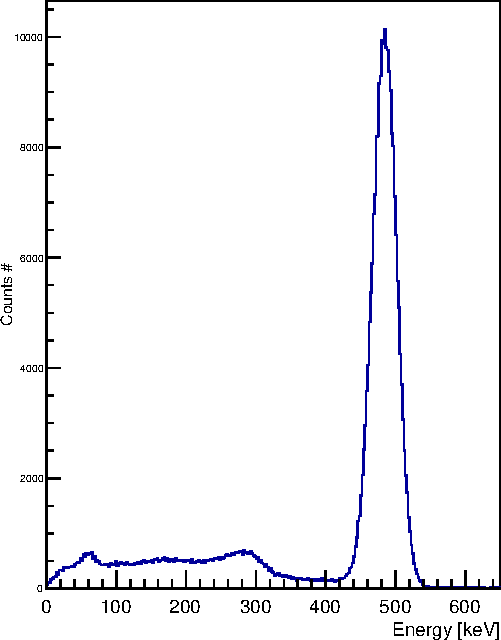
\includegraphics[width=.45\textwidth]{1_2_ch0_origin}} \quad
		\subfloat[][\emph{Detector 2}.]
	{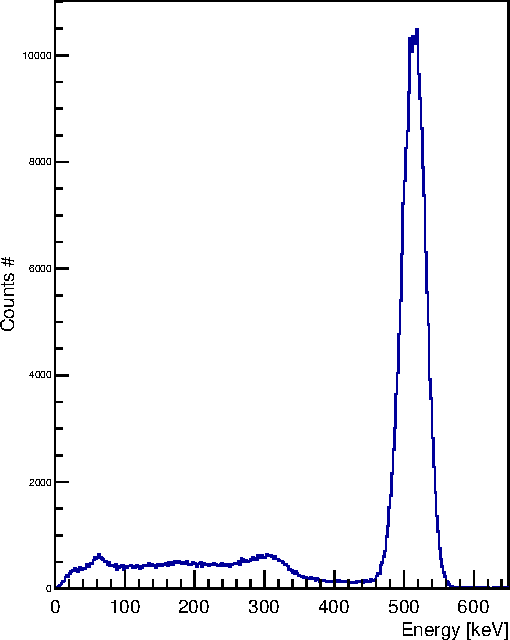
\includegraphics[width=.45\textwidth]{1_2_ch1_origin}} \\
	\caption{Spectra obtained from the two detectors with p-Ps configuration.}
\label{Fig:1_2_spectra}
\end{figure}
In order to determine the number of detected p-Ps decay~($N_{2-\gamma}^{Exp.}$), the photopeak has to be integrated. Therefore the Compton background was removed and an integration window of 3 FWHM width around the photopeak centroid was selected, as presented in Fig \ref{Fig:1_2_integral}.

\begin{figure}[H]
	\centering
	\subfloat[][\emph{Detector 1}.]
	{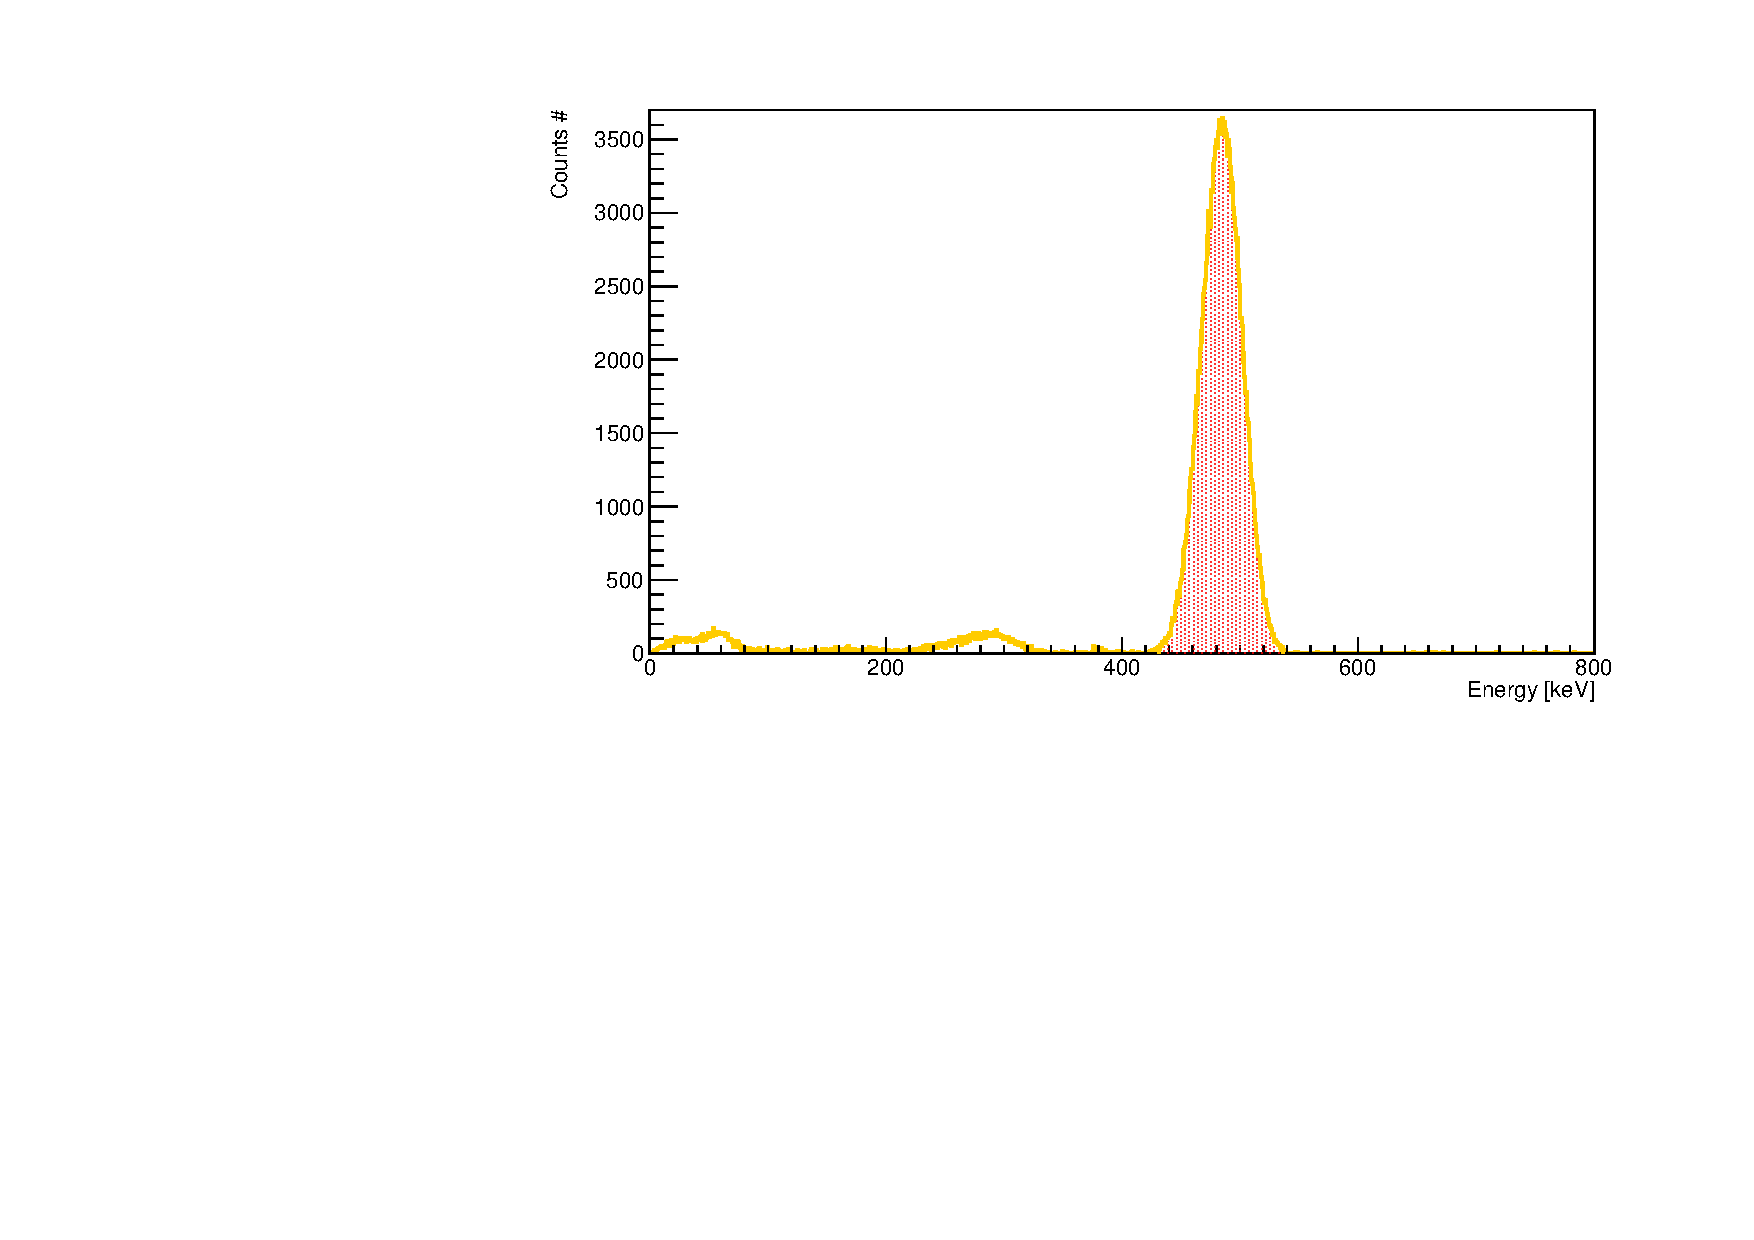
\includegraphics[width=.45\textwidth, height=.20\textheight]{1_2_ch0}} \quad
		\subfloat[][\emph{Detector 2}.]
	{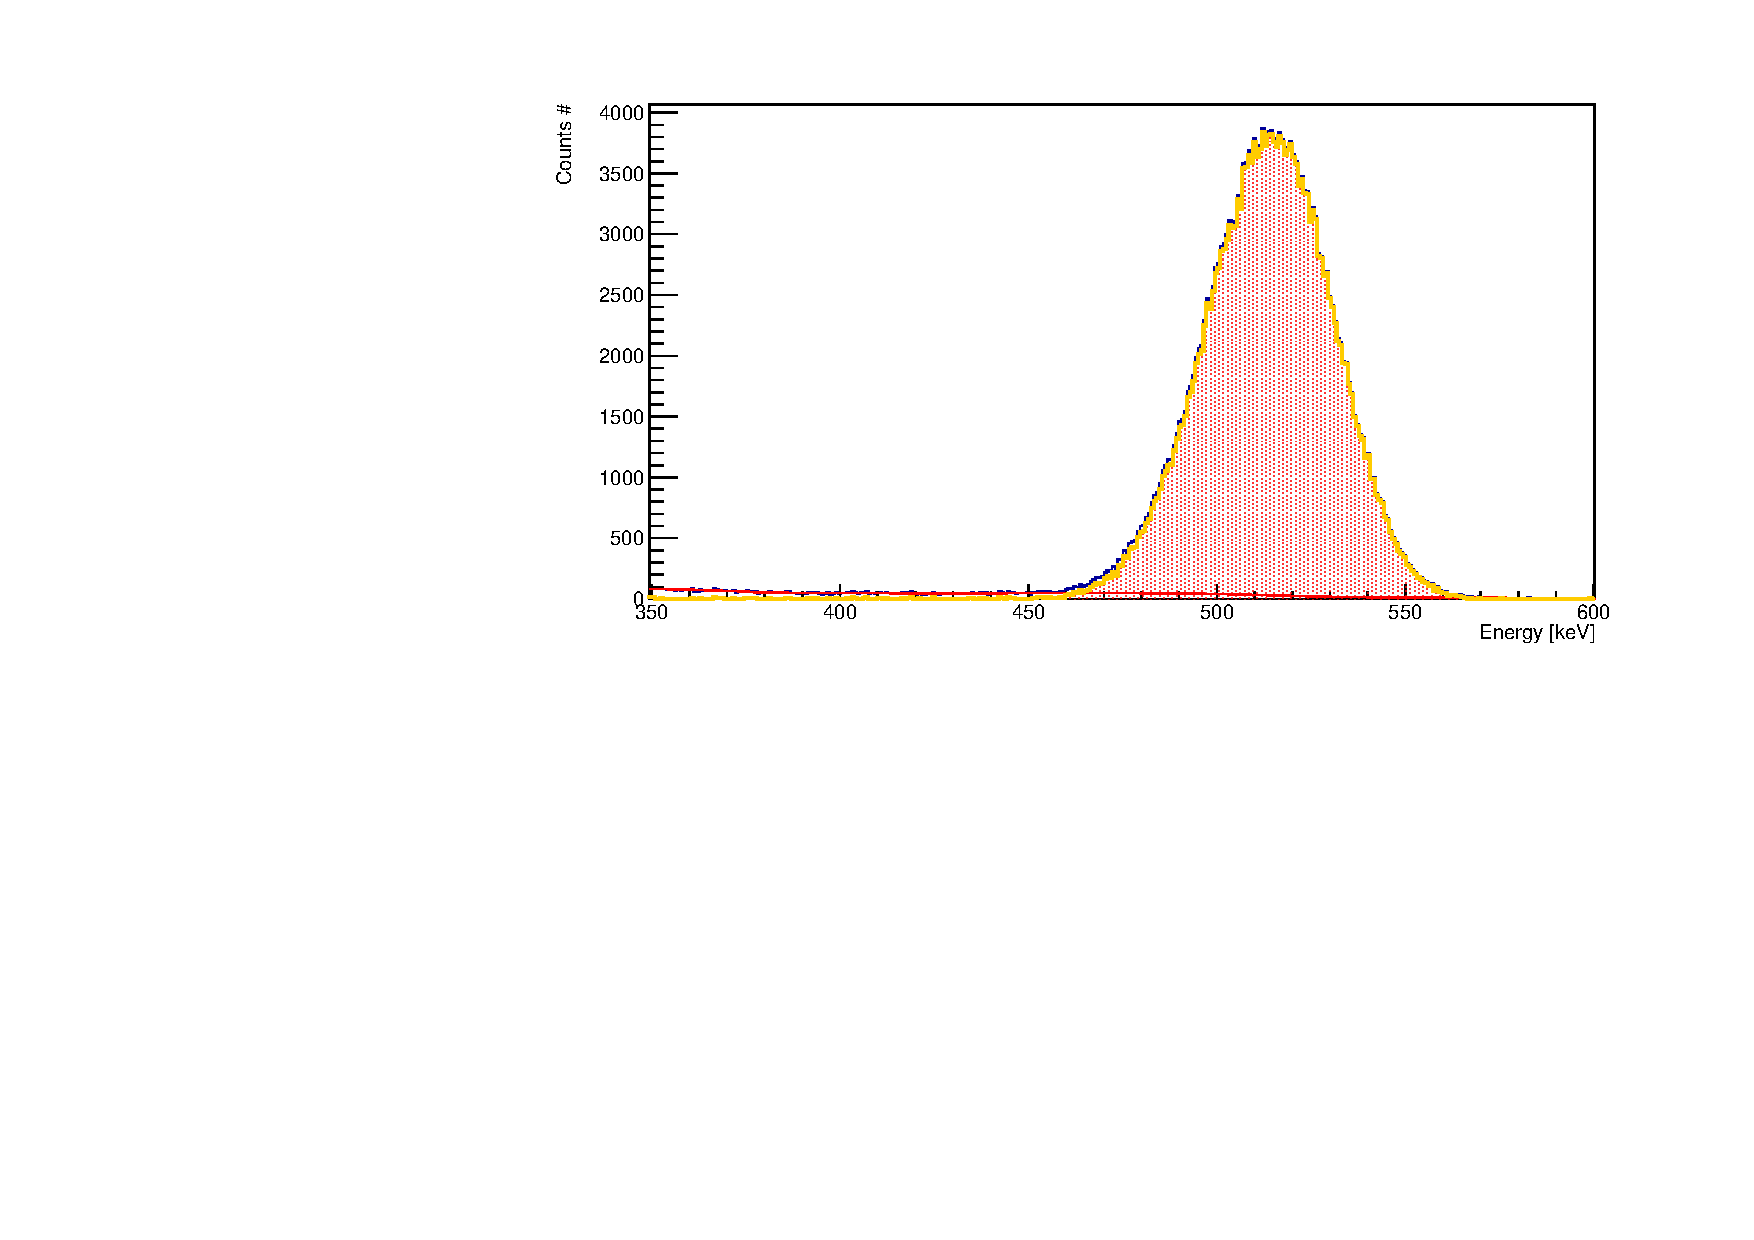
\includegraphics[width=.45\textwidth, height=.20\textheight]{1_2_ch1}} \\
	\caption{Spectra obtained from the two detectors with p-Ps configuration and background removal. The shaded area represents the events counted by the integral of the photpeak. }
\label{Fig:1_2_integral}
\end{figure}
 
The same was performed with the o-Ps measurements counting the events in the peak at 340~keV~($N_{3-\gamma}^{Exp.}$), one third of the total energy, due to the fact the three $\gamma$ have the same energy at 120$^\circ$. The integrated spectra are shown in Fig.~\ 

\begin{figure}[H]
	\centering
	\subfloat[][\emph{Detector 1}.]
	{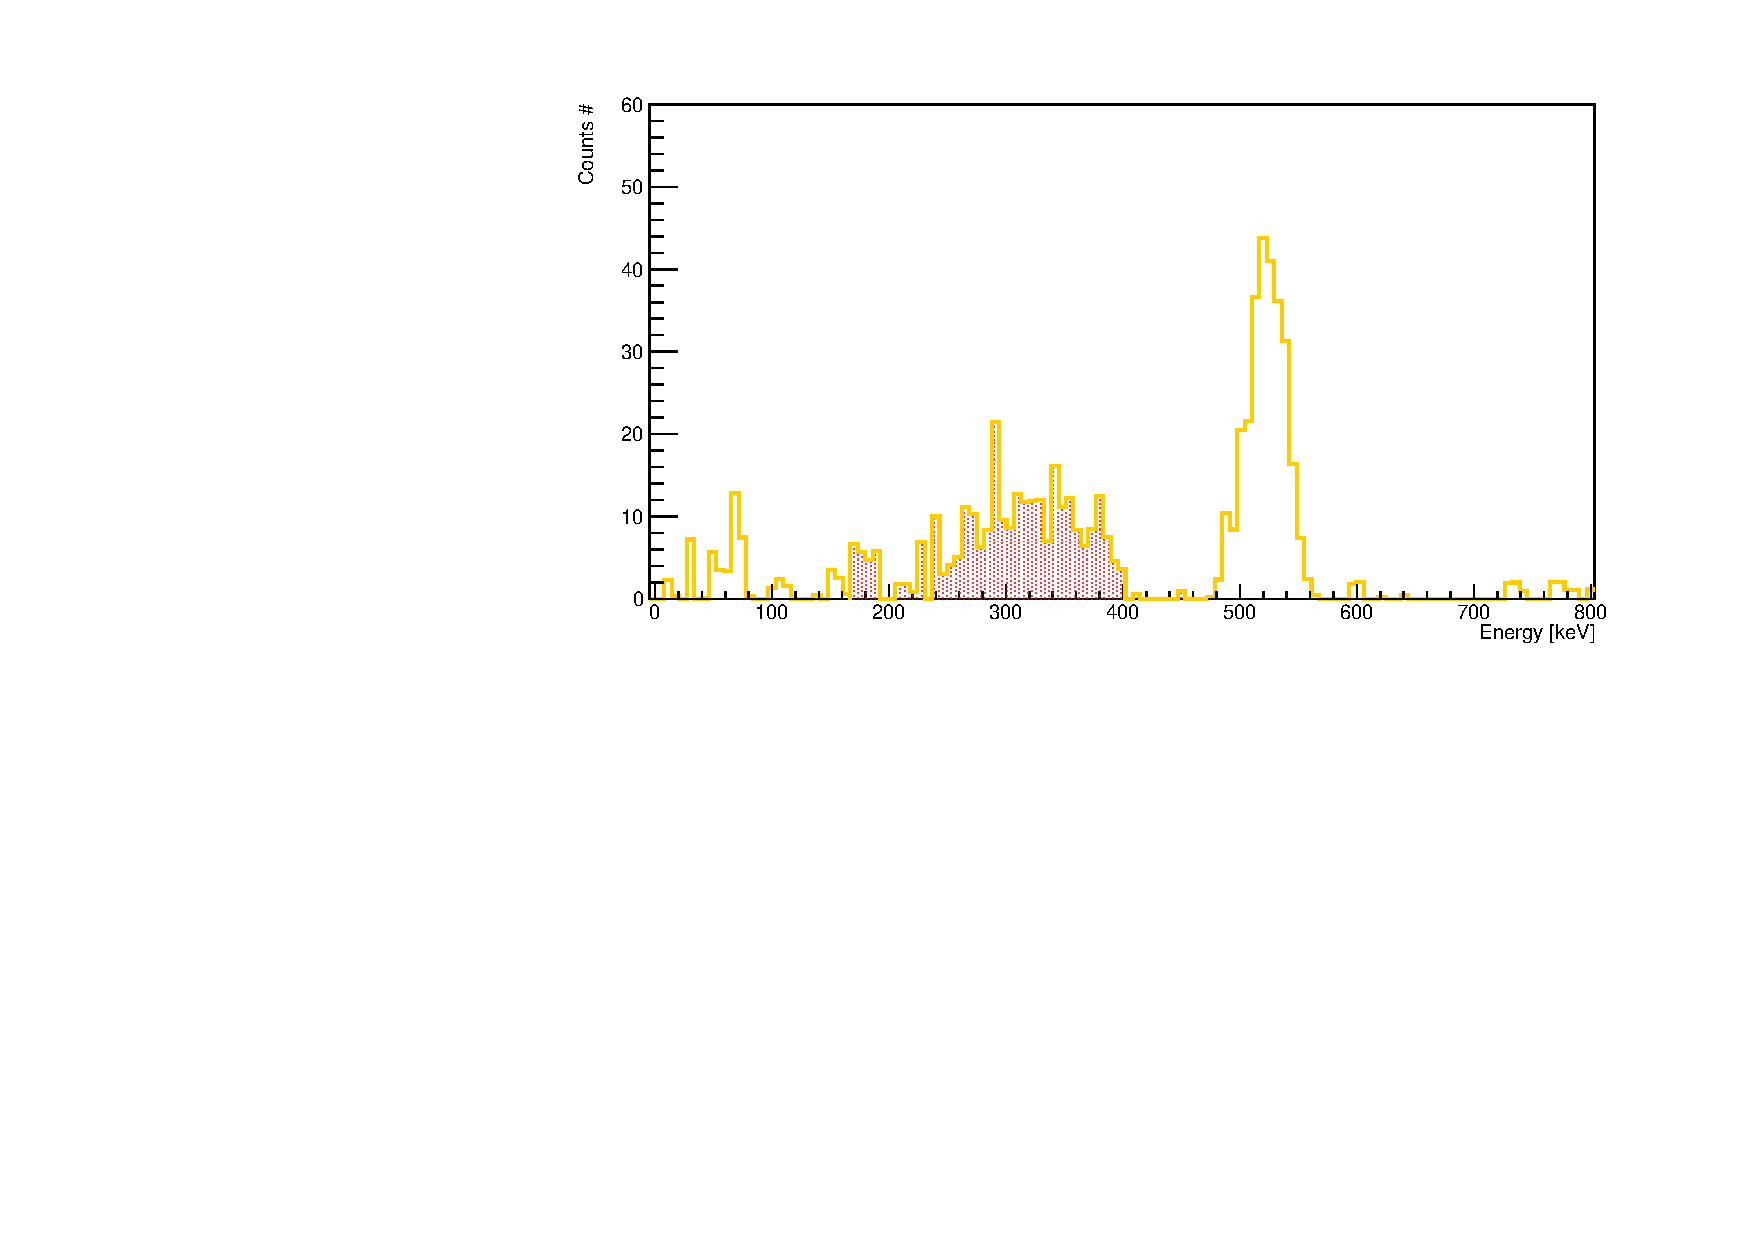
\includegraphics[width=.45\textwidth, height=.20\textheight]{1_2_3_ch0}} \quad
		\subfloat[][\emph{Detector 2}.]
	{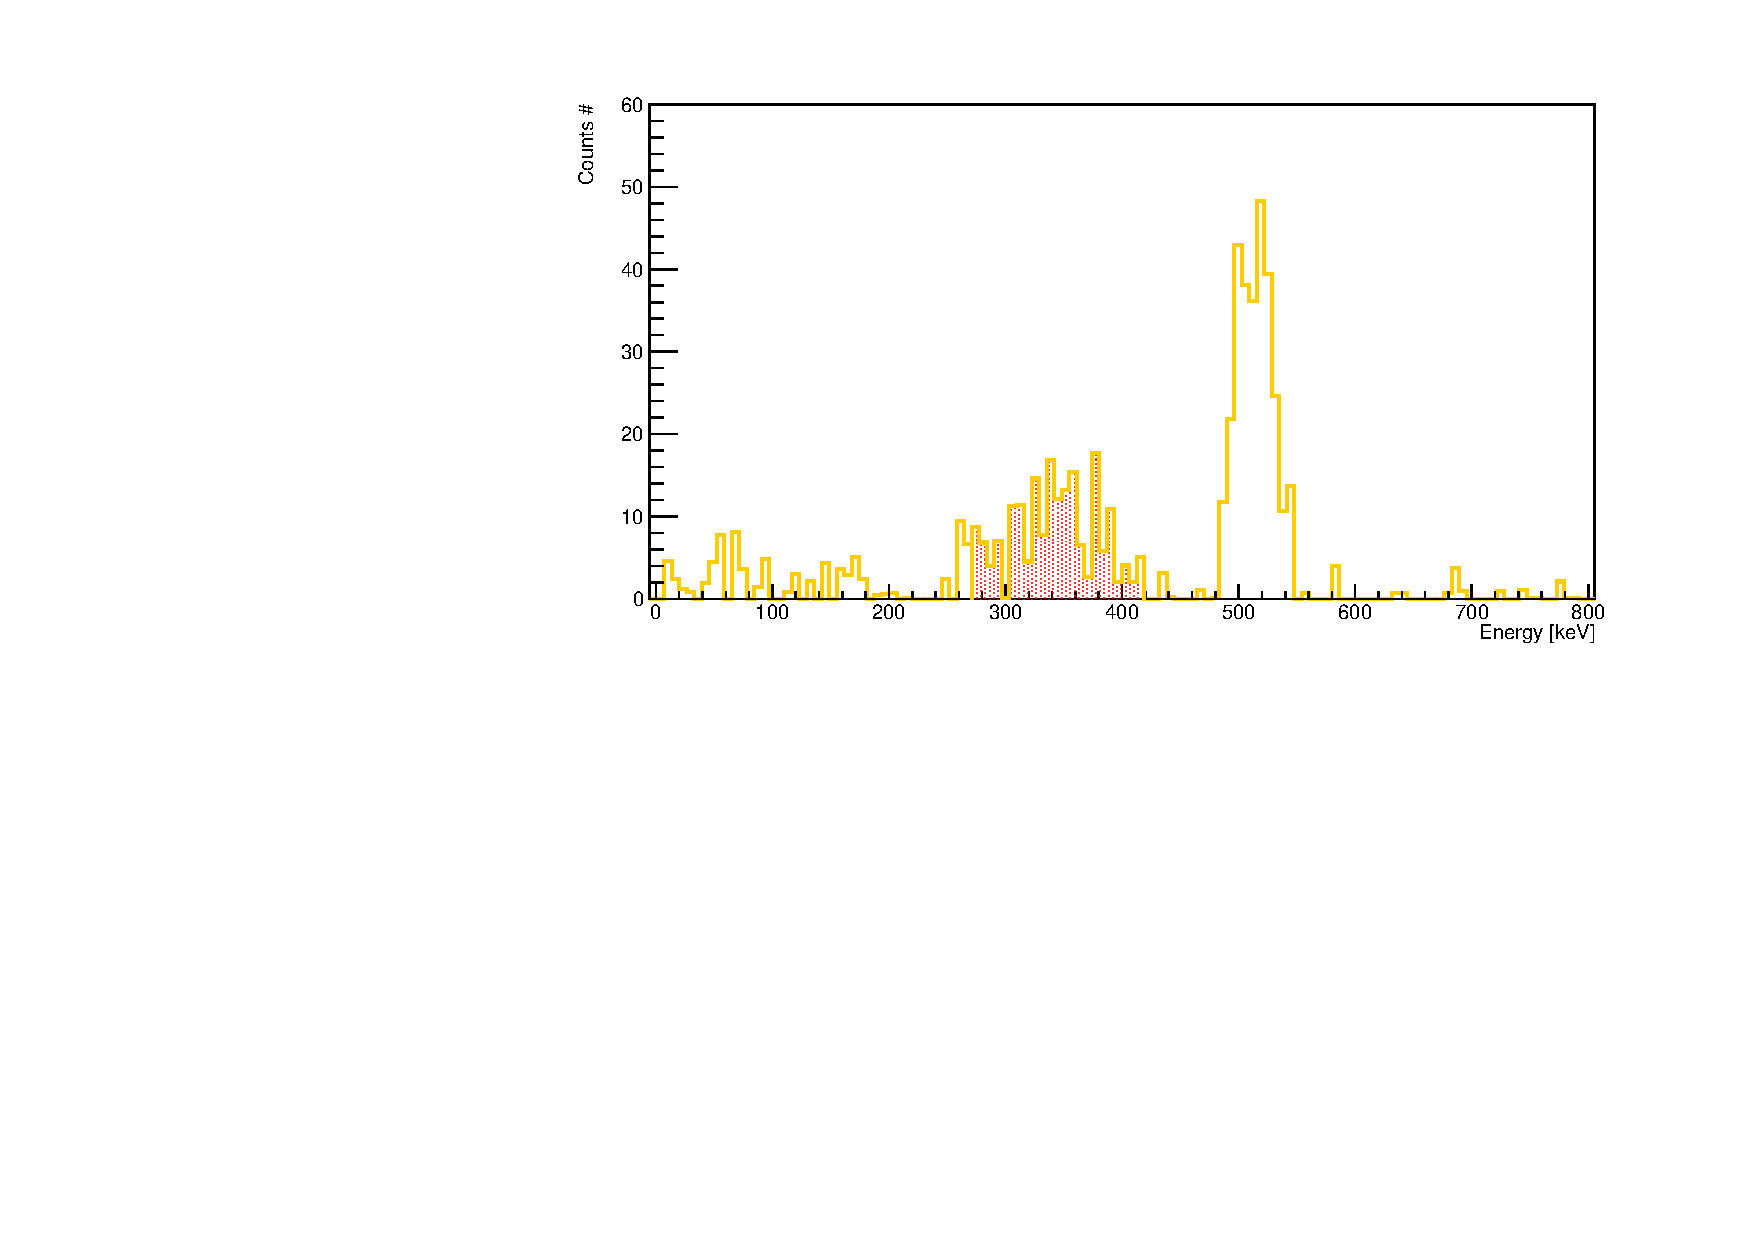
\includegraphics[width=.45\textwidth, height=.20\textheight]{1_2_3_ch1}} \quad
		\subfloat[][\emph{Detector 3}.]
	{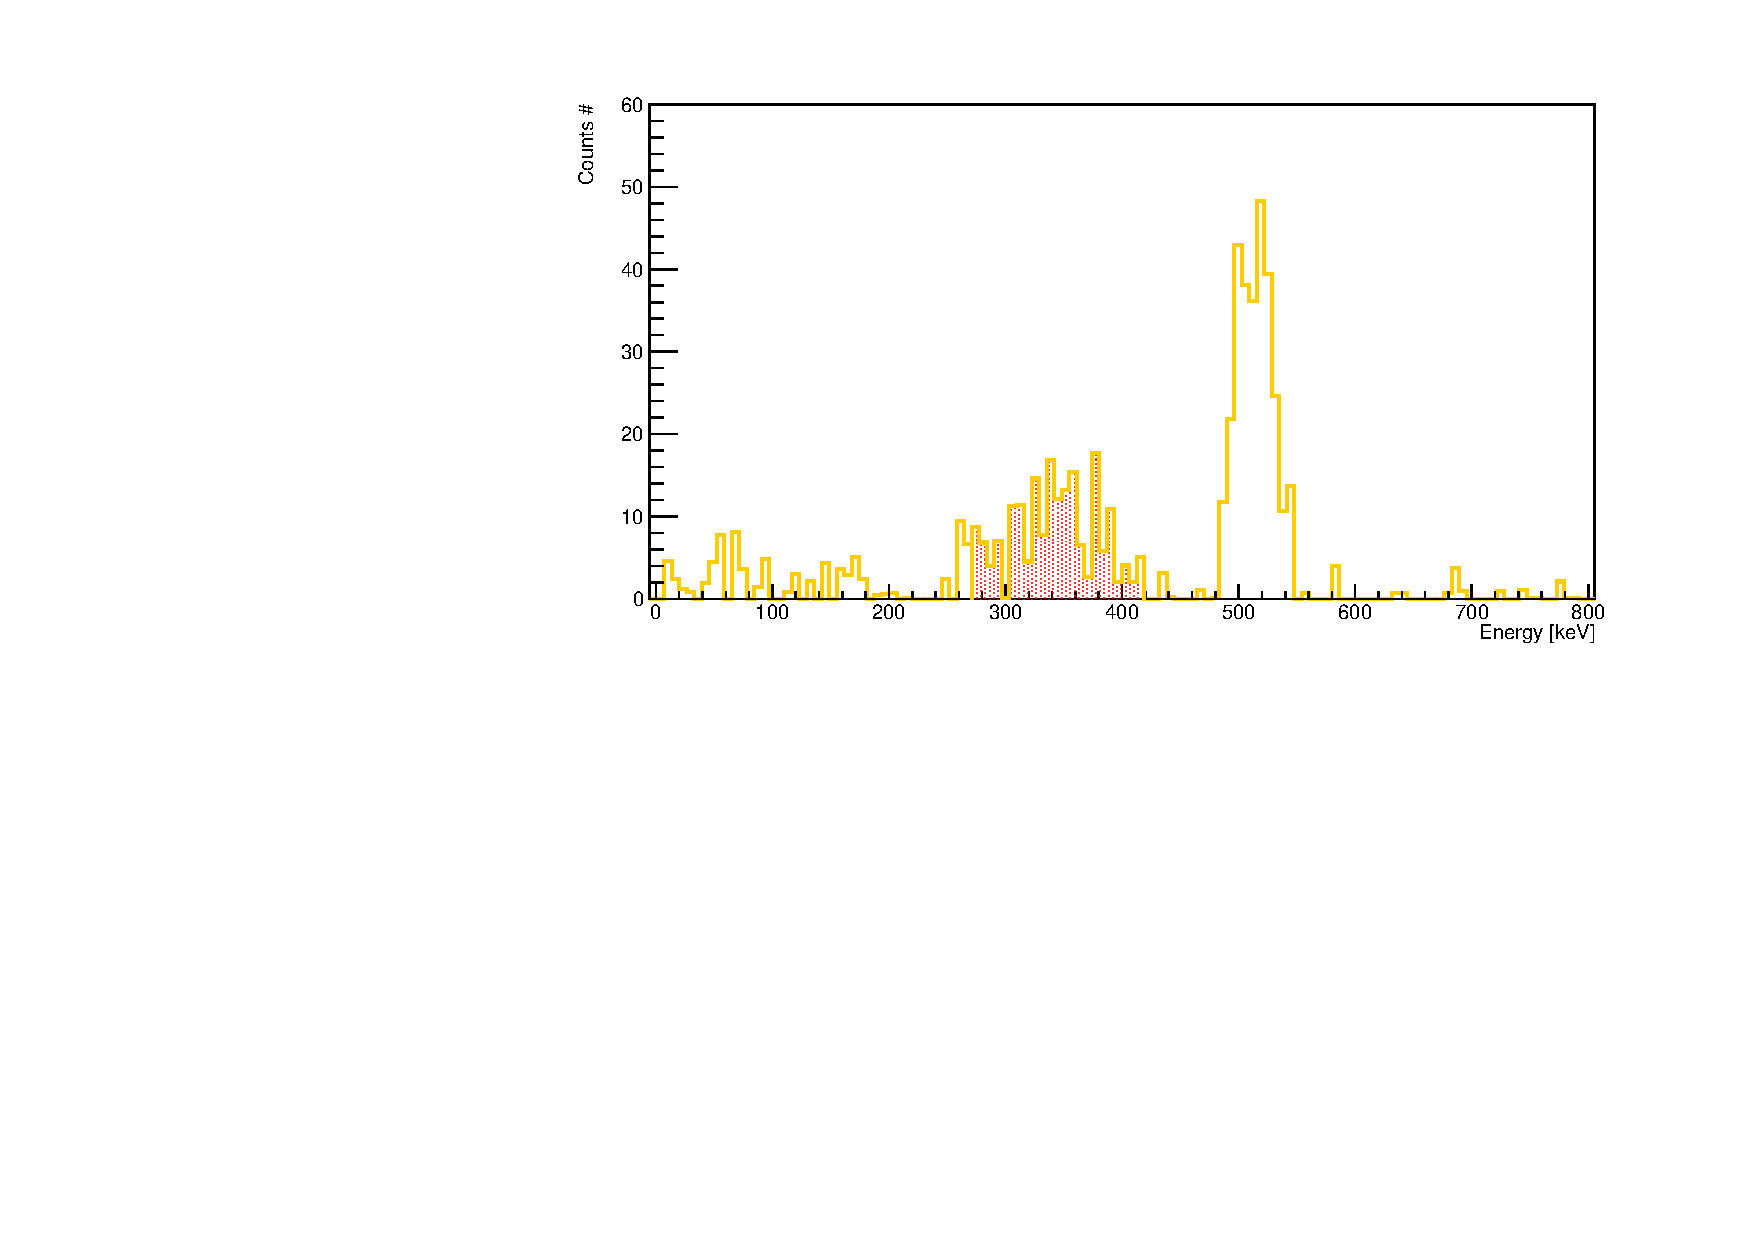
\includegraphics[width=.45\textwidth, height=.20\textheight]{1_2_3_ch1}} \\
	\caption{Spectra obtained from the three detectors with o-Ps configuration and background removal. The shaded area represents the events counted by the integral of the spectrum. }
\label{Fig:1_2_integral}
\end{figure}

The measured counts for the two configuration however are affected by the geometry and efficiency of the system, therefore the following equation was used to correct them and evaluate the branching ratio:
\begin{equation}
Ratio=\dfrac{N_{3-\gamma}^{Tot.}}{N_{2-\gamma}^{Tot.}}=\dfrac{N_{3-\gamma}^{Exp.}\ f_{3-\gamma}^{Geom.}\ \varepsilon_{511~keV}^2}{N_{2-\gamma}^{Exp.}\ f_{2-\gamma}^{Geom.}\ \varepsilon_{340~keV}^3}
\end{equation}

$\varepsilon_{340~keV}$ and $\varepsilon_{511~keV}$ are the detectors intrinsic efficiency at the energies of interest, elevated in the equation to the number of emitted $\gamma$. 

$f_{3-\gamma}^{Geom.}$ and $f_{2-\gamma}^{Geom.}$ are geometric correction factor for the two setup, due to the fact the detectors used in the experiment do not cover the whole solid angle. In the case of $f_{2-\gamma}^{Geom.}$ this is simply the ratio between the surface of the two facing detectors and $4\pi$. The former instead was evaluated performing a simulation, described in the following section. 




